% ======================================================================================================
% TCC - César Henrique Bernabé
% Capítulo 2 - Referencial Teórico
% ======================================================================================================
\chapter{Referencial Teórico}
\label{sec-referencial}

Este capítulo apresenta os principais conceitos teóricos que alicerçaram a evolução do metamodelo de requisitos do \zanshin e de conceitos que fundamentaram o desenvolvimento da ferramenta \unagi. A Seção~\ref{sec-referencial-engenharia-objetivos} fala sobre Engenharia de Requisitos Orientada a Objetivos, destacando os principais conceitos dessa área que foram utilizados ao longo deste trabalho. A Seção~\ref{sec-referencial-zanshin} apresenta o sistema \zanshin e os detalhes do metamodelo original do \framework. A Seção~\ref{referencial-mdd} apresenta um breve resumo sobre Desenvolvimento Dirigido por Modelos (\mdd ou MDD) assim como  as principais ferramentas que foram utilizadas durante o desenvolvimento do \unagi, como as funcionalidades \emf de modelagem do \eclipse, o plugin \sirius, dentre outros.

% ======================================================================================================
% SUBSEÇÃO: Desenvolvimento Dirigido por Modelos
% ======================================================================================================
\section{Desenvolvimento Dirigido por Modelos}
\label{referencial-mdd}
Pesquisadores vêm tentando ao longo dos anos criar abstrações que ajudem programadores a focar no conteúdo do desenvolvimento ao invés das especifidades da tecnologia de criação adotada~\cite{viyovic2014sirius}. O Desenvolvimento Dirigido por Modelos (\mdd ou MDD) pode ser visto como a forma de programação de mais alto nível de abstração existente atualmente~\cite{atkinson2003model}, promovendo o uso de artefatos do processo de desenvolvimento de software para lidar com complexidade por meio de abstração~\cite{viyovic2014sirius}.

Em outras palavras, MDD parte da premissa que um sistema é um modelo consistente com seu metamodelo~\cite{vujovic2014comparative} e, assim, em vez de exigir que programadores escrevam cada simples detalhe da implementação de um sistema, permite que uma funcionalidade necessária para um software possa ser visualmente modelada~\cite{atkinson2003model}. Portanto, essa técnica viabiliza que muitas atividades complexas (porém rotineiras) da área de programação de software sejam automatizadas como por exemplo, o suporte a persistência, interoperabilidade e distribuição~\cite{atkinson2003model}.

A modelagem usa da percepção visual humana para melhorar o processo de compreensão sobre o domínio de um software, já que modelos nos auxiliam a entender problemas complexos e suas possíveis soluções por meio da abstração. Assim, MDD baseia-se na premissa de que o desenvolvimento de software deve focar principalmente na produção de modelos e não na criação de código~\cite{selic2003pragmatics}.

A primeira vantagem dessa abordagem é que podemos usar conceitos mais ligados ao domínio do problema que o software vai resolver, ao invés de focar em conceitos técnicos ligados a linguagem de programação, por exemplo. Essa vantagem acarreta em alguns outros benefícios: modelos são mais compreensíveis do que códigos e portanto, tornam-se também mais fáceis de especificar e manter~\cite{selic2003pragmatics}. Além disso, modelos são menos sensíveis a alterações de tecnologias, ou seja, são independentes de plataforma~\cite{selic2003pragmatics}. 

Esse trabalho usa MDD em vários processos: primeiramente podemos considerar que \zanshin usa das ferramentas desse método para instanciação, validação e outras atividades relacionadas ao modelo do sistema que é fornecido pelo usuário. Segundo, \unagi usa a produção automática de código por meio da interpretação de modelos visuais~\cite{selic2003pragmatics, viyovic2014sirius}, além do que  o processo de modelagem de sistemas e a geração automática dos arquivos \xml para \zanshin também pode ser vista como um processo de \mdd.


% ======================================================================================================
% SUBSEÇÃO EMF
% ======================================================================================================
\subsection{Eclipse Modeling Framework}
O \eclipse é um projeto de código aberto com o objetivo de prover uma plataforma de desenvolvimento altamente integrada. O processo de criação de sistemas no \eclipse pode ser dividido em alguns projetos, entre eles o Projeto de Modelagem (\textit{Modeling Project}), que concentra-se em tecnologias baseadas no desenvolvimento orientado a modelos~\cite{steinberg2008emf}. Esse ambiente é chamado de \textit{Eclipse Modeling Framework} ou \textit{EMF}, e provê funcionalidades como transformação de modelos, integração de bases de dados e geração de editores gráficos~\cite{steinberg2008emf}. Modelos especificados dentro do contexto \emf relacionam abstrações de modelagem diretamente a seus conceitos de implementação, sendo a união das tecnologias \uml, \xml e \java, permitindo a conversão automática entre todas essas~\cite{steinberg2008emf}. 

A tecnologia \emf pode ser melhor explicada com um exemplo: um sistema de gerenciamento de ordem de compras de uma loja, que necessita incluir casos como ``cobrar'' e ``entregar'' em um endereço e uma coleção de itens (nesse caso, compras). A Figura~\ref{exemplo-uml} mostra o diagrama do sistema em \uml. Esse modelo pode também ser descrito dentro do \emf usando modelos \ecore, como na Figura~\ref{exemplo-ecore}. Modelos \ecore são basedos no metamodelo para especificação exibido na Figura~\ref{metamodelo-ecore}, onde classes são representadas por \texttt{EClass}, atributos por \texttt{EAttribute}, relações por \texttt{EReference} e tipos de dados por \texttt{EDataType}. Assim, a ``conversão'' do modelo \uml para \ecore é dada ao se instanciar classes de \ecore de acordo com a especificidade do domínio do problema~\cite{steinberg2008emf}, como pode ser visto na Figura~\ref{exemplo-uml-to-ecore}. 

\begin{figure}
	\centering
	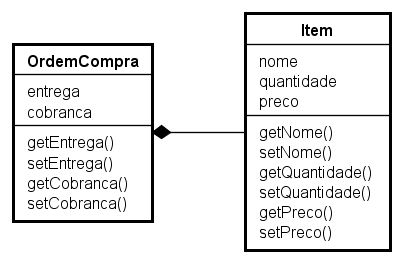
\includegraphics[width=0.65\textwidth]{figuras/exemplos-emf/exemplo-uml.png}
	\caption{Classes do diagrama do exemplo em \uml.}
	\label{exemplo-uml}
\end{figure}

\begin{figure}
	\centering
	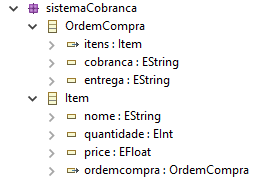
\includegraphics[width=0.6\textwidth]{figuras/exemplos-emf/exemplo-ecore.PNG}
	\caption{Classes do diagrama do exemplo em \ecore.}
	\label{exemplo-ecore}
\end{figure}

\begin{figure}
	\centering
	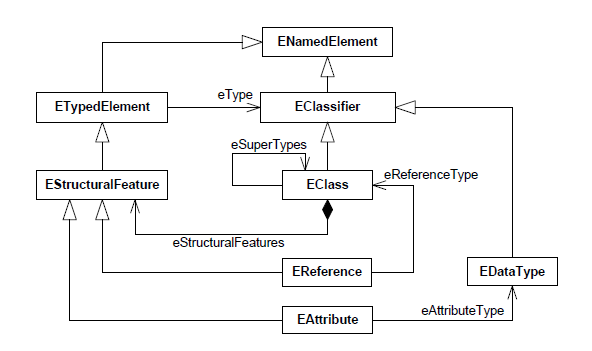
\includegraphics[width=0.95\textwidth]{figuras/exemplos-emf/metamodelo-ecore.png}
	\caption{Metamodelo de \ecore~\cite{kern2008interchange}.}
	\label{metamodelo-ecore}
\end{figure}

Assim que o modelo é detalhado em \ecore, o \emf está pronto para gerar código automaticamente, por meio dos seguintes passos:

\begin{itemize}
	\item Para cada tipo \texttt{EClass} cria-se uma interface e sua classe de implementação correspondente. No caso do exemplo, para a classe \texttt{OrdemCompra} seriam criadas a interface \texttt{OrdemCompra} e a classe \texttt{OrdemCompraImpl}. Essa especificação permite que sejam implementadas funções de persistência e distribuição, porém não serão discutidas aqui por fugirem do escopo desse trabalho.
	\item As classes do tipo \texttt{EAtributte} são transformadas em atributos nas classes correspondentes
	\item As classes tipo \texttt{EReference} são transformadas em referências nas respectivas classes que referenciam.
\end{itemize}

\begin{figure}
	\centering
	
\includegraphics[width=1\textwidth]{figuras/exemplos-emf/uml-to-ecore.png}
	\caption{Conversão do diagrama de exemplo de \uml para \ecore.}
	\label{exemplo-uml-to-ecore}
\end{figure}

Em suma, o \framework de modelagem do \eclipse permite que usuários criem modelos apoiados em metamodelos, e baseando-se no modelo criado, gera partes de código de sistema~\cite{vujovic2014comparative}.

%https://books.google.com.br/books?id=sA0zOZuDXhgC&lpg=PT23&ots=2IQIWZWqNm&dq=eclipse&lr&hl=pt-BR&pg=PT45#v=onepage&q=eclipse&f=false

% ======================================================================================================
% SUBSEÇÃO Sirius
% ======================================================================================================
\subsection{Sirius}

O \sirius é um plugin que simplifica o \framework de Modelagem Gráfica (\textit{Graphical Modeling Framework} ou \textit{GMF}) do \eclipse, reduzindo a complexidade de uso do mesmo e permitindo a produção de editores gráficos de modelos personalizados~\cite{viyovic2014sirius}. O \sirius é construído em cima das utilidades para (des)serialização de modelos, checagem de condições e geração de editores baseados em \ecore providas pelo \eclipse~\cite{budinsky2004eclipse}. Representações criadas com \sirius podem ser apresentadas em diagramas, tabelas e árvores~\cite{viyovic2014sirius}. Em síntese, \sirius provê ferramentas que permitem a especificação de um modelo de um domínio qualquer em diferentes perspectivas gráficas~\cite{vujovic2014comparative}.

Por meio de modelos de especificação (\textit{Viewpoint Specification Model} ou VSM), o \textit{plugin} permite especificar a estrutura, aparência e comportamento do metamodelo do editor a ser criado~\cite{viyovic2014sirius}. Os VSMs são especificados em arquivos \textit{.odesign}~\cite{viyovic2014sirius}, e baseam-se no metamodelo de domínio descrito em \ecore. Um exemplo de caracterização de representação de modelos é mostrado na Figura~\ref{exemplo-sirius}.

\begin{figure}
	\centering
	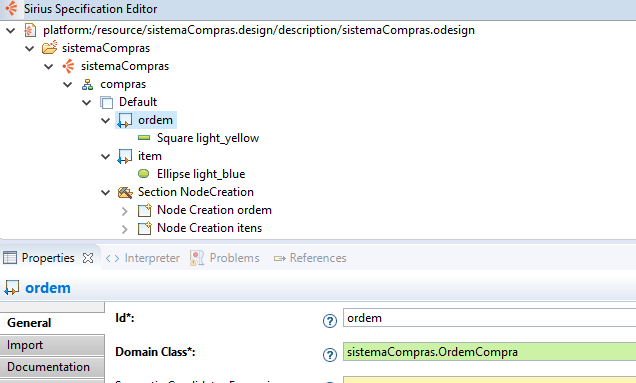
\includegraphics[width=0.9\textwidth]{figuras/exemplos-emf/exemplo-sirius-vsm.png}
	\caption{Exemplo de \textit{Viewpoint Specification Model}.}
	\label{exemplo-sirius}
\end{figure}

\sirius provê vários mecanismos que auxiliam no gerenciamento da complexidade de modelos~\cite{madiot2015eclipse}:

\begin{itemize}
	\item \textbf{Camadas}: é possível separar elementos em camadas diferentes, e ativá-las ou desativá-las.
	\item \textbf{Filtros}: exibir ou esconder elementos dependendo de determinada condição.
	\item \textbf{Personalização de Estilos}: permite modificar propriedades gráficas de elementos do diagrama.
	\item \textbf{Regras de Validação}: permite que a qualidade do modelo seja avaliada.
\end{itemize}


% ======================================================================================================
% SEÇÃO Engenharia de Requisitos Orientada a Objetivos
% ======================================================================================================

\section{Engenharia de Requisitos Orientada a Objetivos}
\label{sec-referencial-engenharia-objetivos}

% Engenharia de Software
A Egenharia de Software é uma área da Ciência da Computação voltada ao estudo dos processos, métodos, técnicas, ferramentas e ambientes de suporte ao desenvolvimento de software, apoiando-se principalmente nas práticas e aplicações da área de Gerência de Projetos com o objetivo de promover melhor organização, produtividade e qualidade em todo o processo de desenvolvimento de um software~\cite{falboEngSoft}.

% Engenharia de Requisitos
Dentro da área de Engenharia de Software, destaca-se uma importante subárea, a área de Egenharia de Requisitos de Software, focada no processo de elicitação de requisitos, considerados fatores determinantes no sucesso do desenvolvimento de um software~\cite{falboEngReq}. Requisitos podem ser entendidos como a definição do que o sistema pode prover, ou também entendidos como o que o sistema é capaz de fazer para atingir um determinado objetivo~\cite{pfleeger2004engenharia}.

% Objetivos
Requisitos estão diretamente ligados aos objetivos do sistema, portanto destaca-se também a Engenharia de Requisitos Orientada a Objetivos, uma subárea da Engenharia de Requisitos. Objetivos são parte importante do processo de elicitação de requisitos, seu propósito é indicar as principais necessidades que justificam a criação de um determinado sistema, demonstrando os casos em que as funcionalidades do mesmo satisfarão as necessidades elicitadas, além de dizer como o sistema deve ser construído para satisfazê-las~\cite{ross1977structured}. 

Em uma descrição geral e resumida do processo de identificação de objetivos, pode-se dizer que o potencial software é analisado nos ambientes organizacional, operacional e técnico, onde são identificados os problemas de contexto e as oportunidades de solução desses conflitos. Então, são elaborados com foco na resolução dos pontos identificados e são devidamente refinados. Por fim, requisitos são criados e refinados com o propósito de atenderem a esses objetivos levantados para o sistema. 

Além de apoiar no processo de modelagem de requisitos, objetivos são usados para apoiar outros propósitos, como gerenciamento de conflitos e o processo de verificação~\cite{lapouchnian2005goal}. De acordo com~\citeonline{van2001goal}, eles podem ser reformulados em diferentes níveis de abstração dependendo do tipo de necessidade que o sistema alvo deve atender, abrangendo desde interesses referentes a estratégias de negócios até conceitos técnicos de atividades.

% Importancia Objetivos
A necessidade de uso de objetivos no processo de modelagem de sistemas de software vem se tornando cada vez mais clara a medida que analistas percebem que:
\begin{itemize}
	\item Objetivos provêm critérios claros de completude dos requisitos do sistema, permitindo também que requisitos desnecessários sejam identificados e descartados~\cite{van2001goal};
	
	\item Objetivos facilitam o processo de entendimento dos requisitos pelas partes interessadas~\cite{van2001goal};
	
	\item O uso de objetivos melhora a legibilidade de documentos de especificação de requisitos, pois permite que engenheiros possam enxergar com mais clareza as alternativas de desenvolvimento do sistema, além de facilitar o processo de gerenciamento de conflitos~\cite{van2001goal};
	
	\item Objetivos dirigem parte do processo de elicitação de requisitos, facilitando a identificação de boa parte deles~\cite{lapouchnian2005goal}.	
\end{itemize}

% Hardgoal, Softgoal, Quality Constraint e Domain Assumption
Diferentemente dos requisitos, objetivos podem precisar da cooperação entre diferentes tipos de refinamentos para que sejam atendidos de forma suficiente~\cite{dardenne1993goal}. Em outras palavras, um objetivo diretamente relacionado ao sistema a ser criado torna-se um requisito, enquanto um objetivo sob responsabilidade de um agente  do ambiente (pode ser um usuário ou outro sistema) em que o software será executado torna-se uma Pressuposição de Domínio (ou \textit{Domain Assumption}) e, nesse caso, são satisfeitos devido a uma regra de negócio~\cite{van2001goal, van1998managing}.

Objetivos funcionais podem ser classificados como objetivos rígidos (\textit{Hard Goals}), cujo critério de satisfação pode ser atendido de forma técnica~\cite{dardenne1993goal} (ou seja, podem ter seu estado definido (sucesso ou falha) de acordo com certas condições) e objetivos fracos (\textit{Soft Goals}), que não possuem critérios claros de satisfação, entretanto são úteis quando deseja-se comparar os melhores refinamentos ao objetivo estudado. Para que \textit{Soft Goals} tenham um parâmetro claro de satisfabilidade, são adicionados a eles os Critérios de Qualidade (\textit{Quality Constraints}). Por exemplo, um \textit{Soft Goal} ``Baixo Custo'' pode ser operacionalizado pelo critério de qualidade ``Custo deve ser menor que R\$ 1 mil''.

Por fim,~\citeonline{jureta2008revisiting} definem outro tipo de refinamento para especificar a satisfação de um objetivo: as tarefas (\textit{Taks}), que são os passos a serem tomados para que um determinado objetivo seja cumprido. Em outras palavras, tarefas são definidas por funcionalidades do sistemas que, se executadas com sucesso, são consideradas satisfeitas~\cite{souza2012requirement}.

% Refinamentos
Objetivos relacionam-se uns com os outros por meio de refinamentos. Segundo~\citeonline{dardenne1991goal}, também em~\cite{dardenne1993goal}, objetivos podem ser refinados usando grafos E/OU (\textit{AND/OR}). O critério de satisfabilidade de objetivos refinados em ``E'' ou ``OU'' segue os conceitos da lógica booleana: refinamentos do tipo ``E'' implicam que, para que um objetivo seja considerado satisfeito, todos os sub-objetivos refinados a partir dele devem estar em estado de sucesso, enquanto refinamentos do tipo ``OU'' relacionam o objetivo principal com um conjunto de alternativas, ou seja, basta que um de seus refinamentos seja atendido para que ele também seja considerado alcançado. Objetivos são refinados até atingirem um nível de granularidade em que são refinados apenas em tarefas, que podem ser completadas com sucesso por um ator (humano ou outro sistema)~\cite{souza2013awareness}. No contexto do \zanshin, refinamentos podem acontecer entre Objetivos e outros Objetivos, \sofgoals, Tarefas e Pressuposições de Domínio e por Tarefas em outras Tarefas.

%Representação Gráfica
Em questões de representação gráfica, os modelos de objetivos discutidos nesse texto são grafos ordenados que exibem as exigências das partes interessadas no topo do modelo e, abaixo, objetivos e tarefas mais refinados, adotando uma topologia do tipo árvore. A simbologia utilizada é baseada na sintaxe de \istar~\cite{yu20111}. Um exemplo de modelo de objetivos representando um sistema de despacho de ambulâncias é mostrado na Figura~\ref{figura-acad-simples}.

\begin{figure}
	\centering
	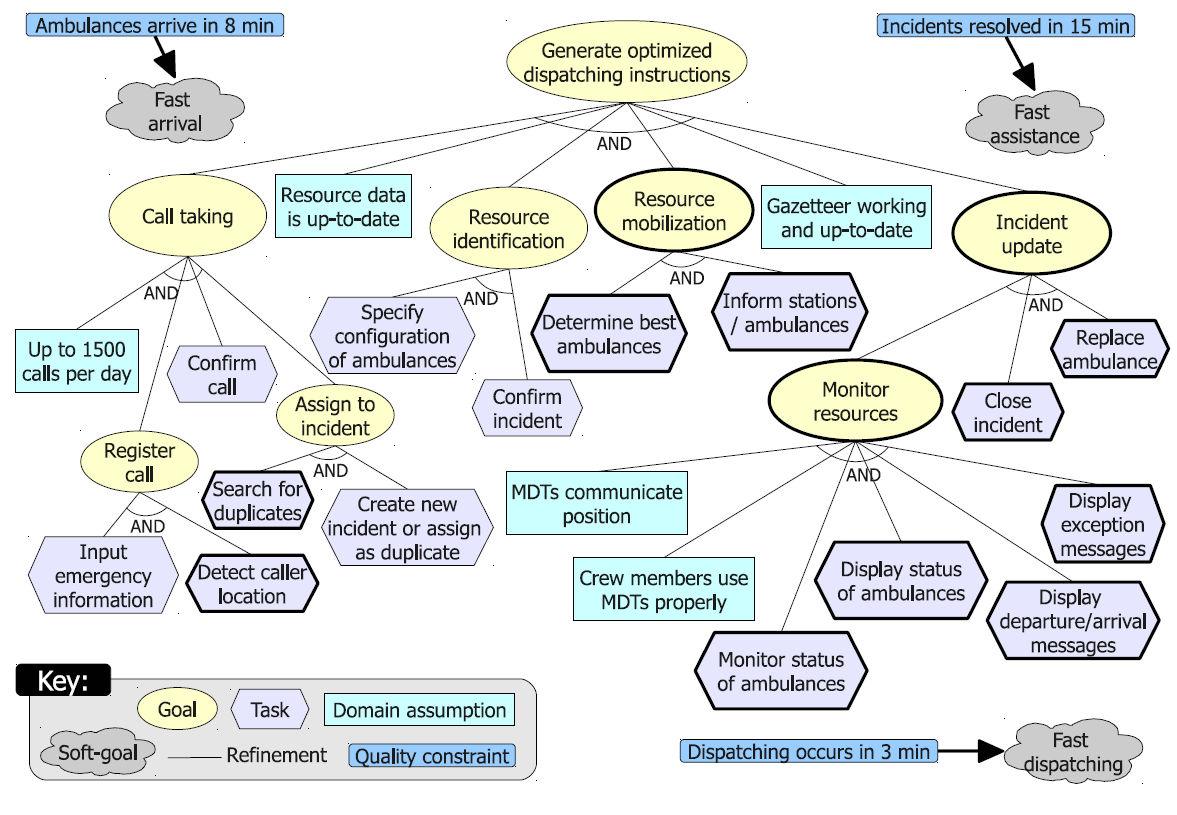
\includegraphics[width=1\textwidth]{figuras/modelos/ACAD-Simples.png}
	\caption{Exemplo de modelos de objetivos~\cite{tesevitor}.}
	\label{figura-acad-simples}
\end{figure}

% ======================================================================================================
% SUBSEÇÃO GORO
% ======================================================================================================
\subsection{GORO}
\label{sec-referencia-engenharia-objetivos-goro}
\goro (\textit{Goal-Oriented Requirements Ontology}) é uma ontologia de referência baseada no domínio de \gore e fundamentada em UFO (\textit{Unified Formal Ontology})~\cite{guizzardi2005ontological}. Uma ontologia pode ser definida como um modelo de dados que representa um conjunto de conceitos relacionados a um domínio específico e também define o relacionamento entre esses conjuntos˜\cite{gruber2009ontology}. Em outras palavras, uma ontologia é uma forma de representação do conhecimento sobre um assunto da realidade. 

\goro foca principalmente no conceito de objetivos, tendo como principal objetivo o esclarecer e explorar a natureza dos conceitos envolvidos, buscando assim aumentar a eficiência da comunicação entre os \textit{stakeholders} de um projeto. 

Essa ontologia foi construída por meio da extração de conceitos de diferentes ontologias, como \istar~\cite{dalpiaz2016istar}, KAOS~\cite{dardenne1993goal}, Techne~\cite{borgida2009techne} e UFO. Assim, os principais elementos de \goro são:

\begin{itemize}
	\item \textbf{Intentions e Desires}: concentram-se na modelagem dos objetivos dos agentes, que são definidos em UFO como algo que existe na realidade e possui uma identidade particular, não tendo partes temporais mas existindo no tempo e existencialmente independente. Agentes possuem propriedades relacionadas a intenção, como Desejos (\textit{Desires}), Crenças (\textit{Beliefs}) e Intenções (\textit{Intentions}). Assim, um objetivo é um conteúdo proposicional relacionado ou à intenção ou ao desejo do agente~\cite{pedrogoro}.
	\item \textbf{Goals e Requirements}: Um requisito é um comportamento desejado, portanto, um requisito é também um objetivo "que descreve as condições ambientais a serem alcançadas por meio de uma solução desejada, resultando na satisfação dos objetivos estratégicos subjacentes"~\cite{pedrogoro}.
	\item \textbf{Hardgoals, Softgoals, Requisitos Funcionais e Não-Funcionais}: Adotando a conceituação de~\cite{guizzardi2014ontological}, \textit{Hardgoals} são definidos em \goro como requisitos que são satisfeitos mediante um dado conjunto de situações, enquanto \textit{Softgoals} referem-se a uma definição vaga de qualidade que só podem ser consideradas satisfeitas mediante julgamento do \textit{stakeholder}. Por fim, Requisitos Funcionais referem-se a funções que podem manifestar determinado comportamento por meio de determinadas situações, enquanto Requisitos Não-funcionais referem-se a qualidades~\cite{pedrogoro}.
	\item \textbf{Assumptions}: referem-se a pressuposições de domínio das quais as partes interessadas acreditam ser uma verdade no domínio do problema.
	\item \textbf{Decomposition, Alternatives, Operationalization e Plans}: \textit{Decomposition} é, como o próprio nome diz, uma decomposição de um Objetivos em Sub-objetivos, assim, diz que um objetivo é satisfeito quando todos os seus sub-objetivos são satisfeitos. Da mesma forma, diz que um objetivo pode ser atingido de diferentes maneiras, sendo essas as alternativas (\textit{Alternatives}) de satisfação daquele. \textit{Operationalization} é um link que conecta um Objetivo a uma Tarefa, e especifica como aquele objetivo deve ser satisfeito por meio da tarefa. Por fim, \textit{Plans} são descritos como uma forma de fazer alguma coisa ou tarefa.	
\end{itemize}

% ======================================================================================================
% SEÇÃO Zanshin
% ======================================================================================================

\section{Zanshin}
\label{sec-referencial-zanshin}

Apresentado por~\citeonline{tesevitor}, \zanshin é um \framework que utiliza de ciclos de retro-alimentação para monitorar sistemas e enviar estratégias de adaptação com base em informações de modelos de requisitos orientados a objetivos enriquecidos com elementos construído especialmente para guiar o processo de adaptação. O nome \zanshin vem do japonês e significa ``estado de completa consciência''.

Em tempo de execução, os elementos do modelo de objetivos são representados por classes e instanciados cada vez que o usuário (ou sistema) busca atingir um objetivo, e então o sistema passa a enviar mensagens a essas instâncias quando há mudança de estado. Percebe-se, assim, que objetivos e pressuposições de domínio não são tratadas como invariantes que devem sempre ser atingidas, já que o sistema pode falhar ao tentar atingir seus objetivos iniciais e, então, o componente de adaptação lidará com essas falhas e tomará medidas para que os objetivos voltem a ser satisfeitos~\cite{souza2013requirements}.

Assim como o monitoramento de objetivos por meio do \textit{Feedback Loop}, o \zanshin também monitora Parâmetros (\textit{Parameters}) que podem ser definidos em dois tipos. Primeiro, os Pontos de Variação (ou \textit{Variation Points}), que representam refinamentos do tipo ``OU'' (\textit{OR}). Segundo, as Variáveis de Controle (ou \textit{Control Variables}), que são abstrações referentes a pontos de variação repetitivos ou usados em grande escala. A especificação do comportamento dessas estratégias é discutido em seções posteriores.

O metamodelo dos modelos de objetivos usados no \zanshin é representado na Figura~\ref{figura-metamodelo-antigo} e especificado no código do \textit{framework} por meio	 de uma tecnologia \ecore para descrição e suporte a modelos em tempo de execução. Nessa caso, o modelo representa os tipos de requisitos em nível de classe~\cite{souza2013requirements}. 

%\vitor{É estranho falar de todas as tecnologias específicas do Eclipse aqui sem ter explicado elas antes. Talvez seja o caso de retomar isto quando você falar de EMF, mais à frente.}

\begin{figure}
	\centering
	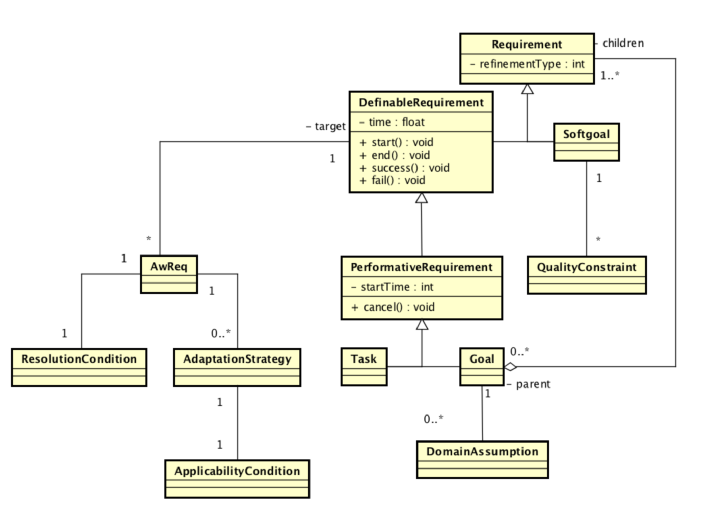
\includegraphics[width=1\textwidth]{figuras/metamodelos/metamodelo-zanshin-antigo.png}
	\caption{Metamodelo que define a sintaxe abstrata para o \zanshin.}
	\label{figura-metamodelo-antigo}
\end{figure}

O \zanshin pode ser dividido em quatro componentes principais, entretanto essa seção foca na discussão de dois desses: o componente de monitoramento e o componente de adaptação.

% ======================================================================================================
% SUBSEÇÃO Modelos de Objetivos em Tempo de Execução
% ======================================================================================================

\subsection{Modelos de Objetivos em Tempo de Execução}
\label{sec-referencial-engenharia-objetivos-runtime}

% Sistemas adaptativos
Muitas vezes os requisitos de um \textit{software} precisam ser modificados durante o ciclo de execução do mesmo. Além disso, ao longo do processo de especificação as partes interessadas no sistema podem apresentar requisitos condicionais, ou seja, que assumem diferentes configurações dependendo da ocorrência de determinada situação~\cite{souza2012requirement}. Em outras palavras, há a necessidade de sistemas que possam se automonitorar e, caso necessário, se adaptar para que seus objetivos continuem sendo satisfeitos~\cite{dalpiaz2013runtime}. Esse tipo de sistema geralmente é composto por duas partes principais: a primeira sendo o sistema em si, que executa uma tarefa para cumprir um objetivo desejado e a segunda sendo um sistema de monitoramento do primeiro, que envia a ele instruções de modificação de suas configurações para que seus objetivos continuem sendo atendidos~\cite{souza2013awareness}. 

O sistema de monitoramento é construído fundamentado na premissa de que todo \textit{software} possui um ciclo de retroalimentação (\textit{feedback loop})~\cite{brun2009engineering} e, assim, o processo de adaptação é realizado com base nesse ciclo, aplicando controladores de resposta que monitoram o comportamento do sistema e enviam estratégias de adaptação~\cite{souza2013awareness}. O módulo adaptador verifica, de acordo com as saídas do sistema alvo, se os objetivos internos a esse estão sendo atendidos e, para isso, necessita importar o modelo de objetivos~\cite{souza2013awareness} enriquecido de elementos que indicam os requisitos a serem observados e as estratégias de adaptação relativas, que serão discutidos adiante.

Modelos de sistemas adaptativos incluem requisitos autoconscientes, ou seja, definidos em relação ao sucesso, falha ou qualidade de serviço de outros requisitos~\cite{souza2013awareness}. Assim, esses são considerados requisitos ``especiais'', já que sua operacionalização está relacionada à mudança de outros requisitos~\cite{souza2012requirement}. Ademais, o comportamento do sistema é caracterizado por eventos que ocorrem em tempo de execução e que estão diretamente ligados a instâncias de objetivos~\cite{dalpiaz2013runtime}. Além disso, é importante observar que essa abordagem é considerada orientada a objetivos já que os requisitos mencionados são derivados do refinamento de objetivos elicitados para o sistema.

%Awreqs
Requisitos autoconscientes são divididos por~\citeonline{souza2012requirement} em dois tipos principais: Requisitos de Percepção (\textit{Awareness Requirements} ou \awreqs)~\cite{souza2013awareness} e Requisitos de Evolução (\textit{Evolution Requirements} ou \evoreqs). \awreqs são requisitos que referem-se ao estado de outros requisitos em tempo de execução, representando situações onde as partes interessadas desejam que o sistema se adapte~\cite{souza2012requirement}, e podem se referir a qualquer tipo de elemento, sejam objetivos, \sofgoals, tarefas ou pressuposições de domínio. Ainda mais, \awreqs indicam o quão critico um requisito pode ser ao descrever o grau de tolerância a falhas do mesmo~\cite{souza2012requirement}. Antes da execução de um sistema, os requisitos estão em estado ``Não Decidido'' (\textit{Undecided}), e então pode assumir os estados ``Sucesso'' (\textit{Succeeded}), ``Falha'' (\textit{Failed}), e no caso de objetivos e tarefas, ``Cancelado'' (\textit{Canceled})~\cite{souza2013awareness}. É fácil notar que o processo de elicitação de requisitos de percepção só acontece depois que o modelo de objetivos é levantado, e assim como o processo de construção de objetivos, \awreqs são sistematicamente criados.

%Evoreqs
\evoreqs são requisitos que modificam o espaço de comportamento do sistema, permitindo que novas alternativas de requisitos sejam usadas, baseando-se em um conjunto pré-definido de etapas de evolução para os requisitos monitorados~\cite{souza2012requirement}. Isto é, \evoreqs são requisitos que especificam uma série de operações primárias em relação a outros requisitos diante de determinadas situações, dizendo ao sistema como adaptar-se~\cite{souza2012requirement}. Instruções para adicionar, remover ou modificar o estado de um objetivo (em nível de instância), desfazer as ações de uma execução que resultou em falha são exemplos de diretivas de adaptação~\cite{souza2013requirements}.

Em suma, \awreqs especificam quando um determinado objetivo precisa de mudanças para continuar a ser atendido, enquanto \evoreqs especificam como executar tais mudanças. A seguir, o modelo de exemplo apresentado na seção~\ref{sec-referencial-engenharia-objetivos} é novamente apresentado, porém com novos requisitos de adaptação que são devidamente discutidos na próxima sessão.

%\vitor{Achei que esta seção (acima) fala mais de Zanshin do que Modelos de Objetivos em Tempo de Execução...}

% ======================================================================================================
% SUBSEÇÃO Exemplo de Caso de Uso
% ======================================================================================================
\subsection{Um Exemplo de Modelo \gore}
\label{sec-referencial-engenharia-objetivos-exemplo}

Na Figura~\ref{figura-acad-completo} é apresentado o modelo visual completo do sistema de despacho de ambulâncias (\textit{Adaptive Computer-aided Ambulance Dispatch} ou \textit{A-CAD}). Nele, observa-se o objetivo principal ``Gerar Instruções de Despacho Otimizadas'', representado por uma oval, que é imediatamente refinado em outros objetivos e em uma pressuposição de domínio (retângulo, vide legenda na Figura~\ref{figura-acad-simples}). O refinamento entre o objetivo raiz e seus filhos imediatos é do tipo ``E'' e portanto, para que o objetivo principal seja considerado satisfeito, todos as suas decomposições de primeiro grau precisam ser satisfeitas. Então, verifica-se que o primeiro nível de refinamento do objetivo principal é composto dos objetivos ``Gerenciar Chamadas'' (\textit{``Call Talking''}), ``Identificação de Recursos'' (\textit{``Resource Identification''}), ``Mobilização de Recursos'' (\textit{``Resource Mobilization''}), ``Obtenção de Mapas'' (\textit{``Map Retrieval''}), ``Receber atualizações sobre o Incidente'' (\textit{``Incident Update''}) e da pressuposição de domínio ``Dados sobre recursos está sempre atualizado'' (\textit{``Resource data is up-to-date''}).

\begin{figure}
	\centering
	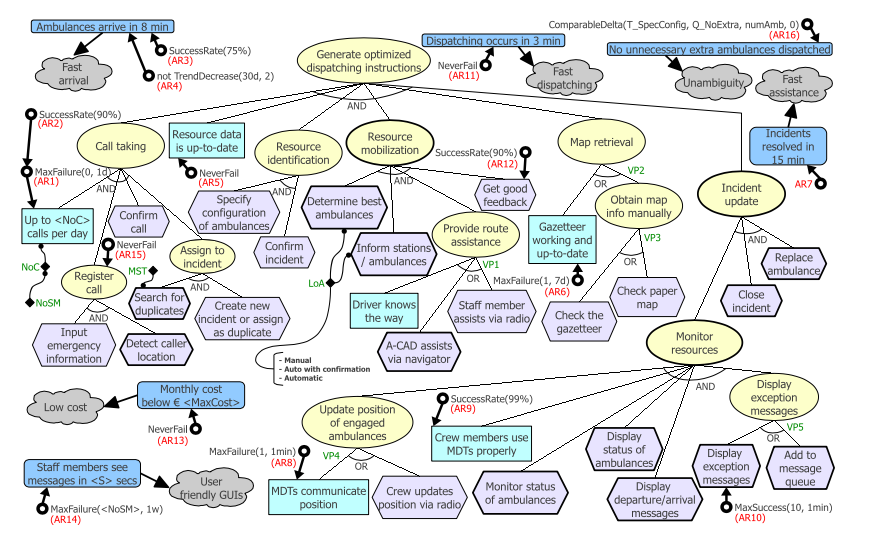
\includegraphics[width=1\textwidth]{figuras/modelos/ACAD-Completo.png}
	\caption{Exemplo de modelos de objetivos de um sistema de despacho de ambulâncias~\cite{tesevitor}.}
	\label{figura-acad-completo}
\end{figure}

O processo de refinamento do modelo então segue até que todos os objetivos sejam completamente decompostos em tarefas ou pressuposições de domínio. \sofgoals são simbolizados por nuvens e refinados em restrições de qualidade representados por retângulos com cantos arredondados. Exemplificando, o \sofgoal ``Chegada Rápida'' (\textit{Fast Arrival}) é operacionalizado por ``Ambulâncias chegam em oito minutos'' (\textit{Ambulances arrive in 8 min}), assim, tem-se um critério claro de satisfação para um objetivo que antes possuía diversos tipos de interpretação, porém, agora, sabe-se que uma ambulância chega rapidamente se consegue estar no local do acidente em menos de oito minutos a partir da chamada.

Os requisitos de percepção são representados por um círculo oco. Por exemplo, o \awreq identificado por ``AR15'', indica que o objetivo ``Registrar Chamados'' deve ``Nunca falhar'' (\texttt{NeverFail}). Os \evoreqs referentes a cada um dos \awreqs não são representados nesse modelo, e devem ser especificados em forma de sequência de operações sobre os elementos do modelo de objetivos (essa escolha de representação visa aprimorar a legibilidade do modelo). Além dos \awreqs, são especificados também os parâmetros de controle (\textit{Control Parameters}), representados por losangos, que indicam parâmetros do sistema que podem ser reconfigurados durante a adaptação. Todas as formas de representação estão resumidas na Figura~\ref{figura-elementos-gore-eca}.

\begin{figure}
	\centering
	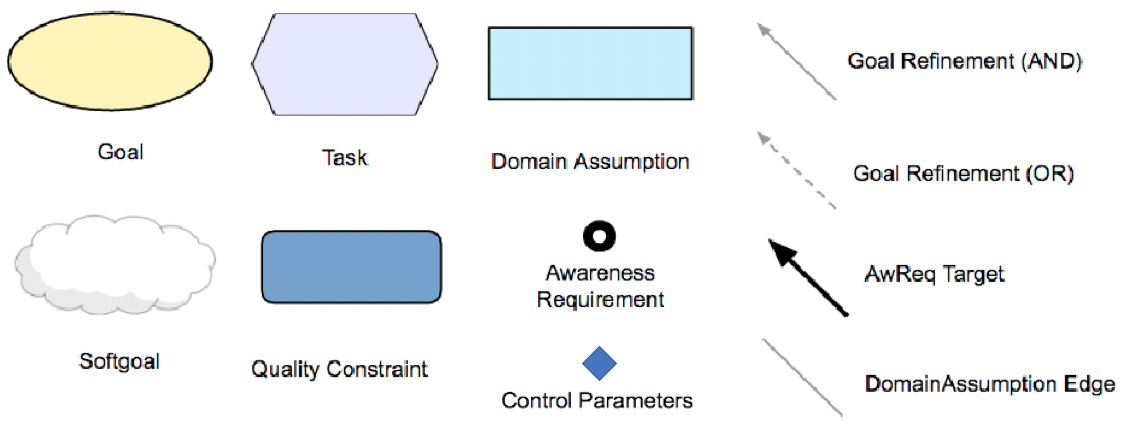
\includegraphics[width=1\textwidth]{figuras/modelos/Elementos-GORE.png}
	\caption{Representação gráfica de elementos de \gore.}
	\label{figura-elementos-gore-eca}
\end{figure}

Sobre os \evoreqs associados ao ``AR15'', podemos definir seus respectivos Requisitos de Evolução. Primeiramente, se o objetivo vir a falhar, define-se a primeira estratégia de adaptação como ``Tentar Novamente em 5 segundos no máximo uma vez'' (\texttt{RetryStrategy(5000)}), caso falhe mais do que uma vez, aplica-se outra estratégia ``Relaxar Condições ao Desabilitar Filho'' (\texttt{RelaxDisableChild(TDetectCaller)}), que desativa o requisito ``Detectar Localização da Ligação'', também aplicado no máximo uma vez. Essas decisões são sumarizadas na Tabela~\ref{tabela-evoreqs-ar15}.

\begin{table}
	\centering
	\caption{Tabela de especificação das estratégias de adaptação de AR15.}
	\label{tabela-evoreqs-ar15}
	\begin{tabular}{|l|l|l|}
		\hline
		AR15 & NeverFail(G\_RegCall) & \begin{tabular}[c]{@{}l@{}}1. Retry(500)\\ 2. RelaxDisableChild(T\_DetectCaller)\end{tabular} \\ \hline
	\end{tabular}
\end{table}

O processo de especificação de como as estratégias de evolução são realizadas pelo sistema é discutido na próxima seção.

%\vitor{Também achei esta seção muito ligada ao Zanshin... Na próxima reunião, vamos conversar sobre uma possível reestruturação, pois vai exigir uma adaptação bem grande na sequência do texto...}

% ======================================================================================================
% SUBSEÇÃO Zanshin: Monitoramento
% ======================================================================================================
\subsection{Monitoramento}
\label{sec-referencial-zanshin-monitoramento}

O módulo de monitoramento necessita que o sistema alvo implemente funcionalidades de registro (\textit{logs}). Por meio do registro, o sistema pode detectar mudanças nos estados das instâncias de um \awreq e assim notificar o serviço de adaptação sobre essas ocorrências. 

Para identificar o modelo de objetivos do sistema alvo, o componente de monitoramento necessita da especificação do modelo do domínio (também em \ecore). Por meio dele, o \zanshin criará instâncias desses objetivos estendendo as classes carregadas do metamodelo de \gore referentes ao tipo de cada um deles (Figura~\ref{figura-metamodelo-antigo}). Por exemplo, ao criar a tarefa ``Especificar configuração de ambulâncias'', o sistema criará uma instancia dessa tarefa específica, que fará referência à classe \texttt{Task} criada no momento em que o metamodelo foi importado. A classe de tarefa especializa a classe \texttt{PerformativeRequirement} que é uma especialização \texttt{DefinableRequirement} (ver Figura~\ref{exemplo-instanciacao-ecore}). 

\begin{figure}
	\centering
	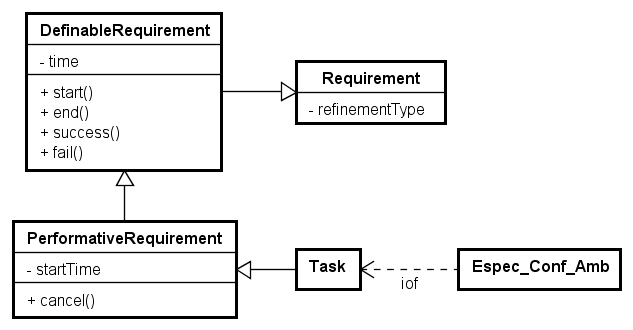
\includegraphics[width=1\textwidth]{figuras/exemplos-emf/exemplo-instanciacao-ecore.PNG}
	\caption{Exemplo de um elemento do modelo de domínio específico instanciado em \zanshin.}
	\label{exemplo-instanciacao-ecore}
\end{figure}

\textit{Performative Requirements} definem os tipos de requisitos que são ou podem ser refinados em tarefas e, assim, possuem ações que são executadas pelo sistema ou seus usuários. \textit{Definable Requirements} são os requisitos que devem possuir um estado definido em algum momento da execução, como por exemplo os objetivos e pressuposições de domínio.

Assim que o \zanshin cria as classes dos requisitos do sistema alvo, o processo de monitoramento apoia-se nos métodos definidos nas metaclasses \texttt{DefinableRequirement} e \texttt{PerformativeRequirement}~\cite{tesevitor} para realizar a monitoração, os métodos disponíveis são:
\begin{itemize}
	\item \texttt{start()}: esse método é chamado nas classes de critérios de qualidade e pressuposições de domínio imediatamente antes da análise de seu estado de satisfação. Para o caso de tarefas, esse método é chamado assim que um usuário inicia uma tarefa, e então todos os ``ancestrais'' desse elemento também têm esse método invocado;
	\item \texttt{success()}: chamado quando um requisito é satisfeito e propagado para todos os pais desse objetivo para ``avisar'' que o filho chegou ao estado de sucesso;
	\item \texttt{fail()}: segue a mesma lógica dos item anteriores, propagando a ``falha'' de um requisito aos seus superiores;
	\item \texttt{cancel()}: para o caso de requisitos como objetivos e tarefas, esse método é usado quando um procedimento é cancelado pelo usuário, usando da mesma lógica de propagação dos métodos anteriores para informar o ocorrido aos pais;
	\item \texttt{end()}: chamado assim que um requisito muda para os estados de sucesso, falha ou cancelamento.
\end{itemize}

Pela descrição dos métodos acima, é possível entender como o processo de monitoramento funciona: basicamente os requisitos monitorados possuem métodos que podem ser chamados em cada caso que assumem, seja de sucesso, falha ou cancelamento. Assim que chamados, os métodos invocam os mesmos procedimentos nos elementos pais, permitindo que a atualização de um requisito se propague a todos os elementos relacionados, atualizando assim todo o modelo.

Logo que o componente monitor detecta uma mudança de estado em um requisito, ou seja, assim que qualquer um dos métodos acima é invocado, ele imediatamente envia uma notificação sobre essa mudança ao módulo de adaptação, que então inicia o processo definido para aquele determinado requisito de percepção~\cite{tesevitor}.

% ======================================================================================================
% SUBSEÇÃO Zanshin: Adaptação
% ======================================================================================================
\subsection{Adaptação}
\label{sec-referencial-zanshin-adaptacao}
Em termos de implementação, o algoritmo do módulo de adaptação cria uma sessão para cada \awreq que está sendo monitorado e então gera uma fila de eventos que se referem a estratégias adaptativas. Assim, essa linha de eventos pode ser usada para verificar se uma estratégia é ou não aplicável a determinada situação. 

Primeiramente, deve-se verificar o estado de um objetivo apontado por um \awreq, para isso é checada a condição de resolução daquele. Então, caso uma avaliação considere que o objetivo está em estado de falha, o sistema segue (de acordo com uma ordem pré-definida) a lista de estratégias de adaptação disponíveis, procurando alguma que tenha sua condição de aplicabilidade verdadeira. Caso encontre, aplica a estratégia definida por aquela condição de aplicabilidade e então retorna ao estado inicial, onde a checagem da satisfabilidade do objetivo é realizada novamente. Caso o objetivo ainda não tenha sido satisfeito, o processo começa novamente, obedecendo restrições como, por exemplo, o número de tentativas de aplicação de uma estratégia, definido individualmente. Caso não encontre uma condição para aplicar uma estratégia, o sistema ativa o método ``abortar'' (\texttt{abort()})~\cite{souza2013requirements}. 

Ao final, quando uma sessão de adaptação é considerada resolvida, a mesma deve ser terminada e, se for necessário que o processo seja aplicado novamente, uma nova sessão é criada. Entretanto, se uma sessão termina sem ter resolvido o problema, o \textit{framework} continuará trabalhando nela do ponto em que parou assim que receber uma nova requisição para adaptação daquele mesmo \awreq. Porém, algumas estratégias também podem forçar que a sessão seja reiniciada quando executada~\cite{souza2013requirements}. Essa processo é conhecido como Evento-Condição-Ação (\textit{Event-Condition-Action} ou \textit{ECA})~\cite{morin2009models}.

% ======================================================================================================
% SUBSEÇÃO Zanshin: ECA
% ======================================================================================================
\subsubsection{ECA}
\label{sec-referencial-zanshin-eca}

O código mostrado na Listagem~\ref{codigo-eca} resume o processo \textit{ECA} para realizar a seleção de estratégias de adaptação:

\begin{lstlisting}[caption={Código do processo ECA},label={codigo-eca}]
processEvent(ar : AwReq) {
	session = findOrCreateSession(ar.class);
	session.addEvent(ar);
	solved = ar.condition.evaluate(session);
	if(solved) break;

	ar.selectedStrategy = null;
	for each s in ar.strategies {
		appl = s.condition.evaluate(session);
		if (appl) {
			ar.selectedStrategy = s;
			break ;
		}
	}

	if (ar.selectedStrategy == null)
		ar.selectedStrategy = ABORT;

	ar.selectedStrategy.execute(session);
	ar.condition.evaluate(session);
}
\end{lstlisting}

O algoritmo da Listagem~\ref{codigo-eca} inicia obtendo a sessão de adaptação referente à classe do \awreq requisitado (caso não haja uma sessão existente, uma nova é criada). Obtida a sessão de adaptação, o algoritmo tem então acesso à lista de eventos de aplicabilidade referentes e, então, adiciona o objeto do \awreq à sessão e imediatamente verifica o estado da mesma (por meio da condição de resolução), parando caso tenha retornado estado de sucesso. Caso contrário, o processo continua procurando por uma estratégia que seja aplicável, checando se a condição de aplicabilidade é verdadeira; caso seja, interrompe o processo e dá à sessão de adaptação uma nova chance de verificar o estado do \awreq. Caso todas as condições sejam falsas e nenhuma estratégia seja selecionada, seleciona a estratégia padrão (\texttt{abort()}) e termina o processo~\cite{tesevitor}. 

Para exemplificar esse processo, tomemos novamente o \awreq ``AR15'', que garante que o requisito ``Registrar chamada'' deve nunca falhar. Caso seja detectado pelo processo de monitoramento que esse requisito apresenta estado de falha, o módulo monitor imediatamente ativa o componente de adaptação, que segue o processo ECA para aplicar estratégias ao ``AR15''. Pelo fragmento de \xml mostrado na Listagem~\ref{listagem-estrategias-AR15}, vê-se que a condição de resolução desse requisito é do tipo \texttt{SimpleResolutionCondition} (considera o objetivo solucionado de acordo com o estado de seus filhos), e que a primeira estratégia a ser selecionada é \texttt{RetryStrategy}, ou seja, tentar novamente (em 5s, de acordo com a propriedade \texttt{time}), entretanto essa estratégia possui a condição de aplicabilidade \texttt{MaxExecutionsPerSessionApplicabilityCondition}, o que significa que ela só pode ser aplicada um determinado número de vezes naquela sessão (nesse caso apenas uma vez, de acordo com o atributo \texttt{maxExecutions}). Caso essa condição seja falsa, a próxima estratégia refere-se a desativar um dos filhos desse objetivo (\texttt{RelaxDisableChildStrategy}), no caso a tarefa ``Detectar localização da chamada'', e possui a mesma condição de aplicabilidade. Se nenhuma dessas condições puderem ser satisfeitas o sistema aborta e, caso contrário, seleciona a primeira estratégia aplicável e verifica novamente o estado do objetivo. A condição \texttt{SimpleResolutionCondition} dita que um objetivo é satisfeito apenas se seus filhos estiverem em estado de sucesso (respeitando a regra booleana do refinamento). 

\begin{lstlisting}[caption={Estratégias de adaptação de AR15},label={listagem-estrategias-AR15}]
<awreqs xsi:type="acad:AR15">										
	<condition xsi:type="eca:SimpleResolutionCondition"/>
		<strategies xsi:type="eca:RetryStrategy" time="5000">
			<condition xsi:type="eca:MaxExecutionsPerSessionApplicabilityCondition" maxExecutions="1"/>
		</strategies>
		<strategies xsi:type="eca:RelaxDisableChildStrategy" child="//@rootGoal/@refinements.0/@refinements.0/@refinements.1">
			<condition xsi:type="eca:MaxExecutionsPerSessionApplicabilityCondition" maxExecutions="1"/>
		</strategies>
</awreqs>
\end{lstlisting}

É importante salientar que as classes referentes a estratégias de adaptação, assim como as condições de aplicabilidade e resolução podem ser estendidas para casos mais complexos, envolvendo inclusive a interação humana~\cite{tesevitor}. Uma lista completa das estratégias de adaptação disponíveis por padrão no \zanshin é mostrada na Tabela~\ref{awreqs-zanshin}.

\begin{table}
	\centering
	\caption{Tabela de Requisitos de Adaptação.}
	\label{awreqs-zanshin}
	\begin{tabularx}{\textwidth}{|l|X|}
		\hline
		\textbf{Regra}                              & \textbf{Efeito}                                                                          \\ \hline
		Abort()                            & Sistema deve falhar de forma prevista, exibindo mensagem de falha, por exemplo. \\ \hline
		Delegate(a)                        & Delegar tarefa a um outro ator do sistema.                                      \\ \hline
		RelaxDisableChild(r, l, child)     & Para de considerar o estado de um requisito em determinada execução do sistema. \\ \hline
		Replace(r, copy, l, newReq)        & Substitui requisito.                                                            \\ \hline
		Retry(copy, time)                  & Tenta novamente em determinado período de tempo.                                \\ \hline
		StrengthenEnableChild(r, l, child) & Volta a considerar estado de um requisito.                                      \\ \hline
		Warning(a)                         & Avisa um ator sobre o estado atual do sistema.                                  \\ \hline
	\end{tabularx}
\end{table}

%For example, the trivial case is considering the problem solved if the (next) AwReq evaluates to success, but this abstract class can be extended to provide di↵erent kinds of resolution conditions, including, e.g., involving a human-in-the-loop to confirm if the problem has indeed been solved, organizing conditions into AND/OR-refinement trees (like in a goal model), etc.


% ======================================================================================================
% SUBSEÇÃO Acceleo
% ======================================================================================================
\subsection{Acceleo}

Acceleo é usada para processos de Transformação de Modelo para Texto (\textit{Model to Text Transformation} ou \textit{M2T})~\cite{acceleouserguide} e, apesar de ser uma linguagem de script, permite integração com linguagens de alto-nível, como por exemplo \java~\cite{mtsweni2012exploiting}. Assim também, Acceleo permite a criação de geradores automáticos de código, usando padrões e \textit{templates}. Em adição, a linguagem é compatível com o ambiente \eclipse e possui um editor próprio dentro do \framework, contando com funcionalidades como destaque de sintaxe, detecção de erros e refatoramento~\cite{WikiAcceleo}. 

Criada em 2005, a linguagem é definida pelos autores do projeto como uma implementação pragmática do modelo \textit{MOF Model to Text Transformation Language}, que é uma especificação para linguagens de transformação de modelos para textos criado pelo \textit{Object Management Group} (\textit{OMG})~\cite{SiteAcceleo}.

%\vitor{Com relação à Seção~\ref{referencial-mdd} como um todo, acho que pode resolver a questão da reestruturação colocada anteriormente se você falar primeiro de MDD, depois de Engenharia de Requisitos.}